\chapter{Automotive - State of art}

Self driving cars are one of the hottest topics of the decade. Artificial Intelligences specifically trained to drive with machine learning techniques demonstrated that it's possible for a computer to drive cars. However, a failure in these kind of systems may have very serious consequences that could result in people being injuried, or killed. At the same time, it is a problem to certify the ultra-high dependability requirements of these systems. In this chapter, today's problems regarding the safety issues related to self driving cars are reviewed, for that it was decided to conduct this study.

\section{Autonomous Cars as CPS}

In order for a car to be able to drive by itself, suitable hardware and software are required. This makes autonomous cars cyber physical computer systems, and the possible catastrophic consequences that a failure in/of these systems can cause, make them fall under the set of critical systems.\newline

To sense and map the surrounding environment, the system collects data from multiple sensors. Some of the most important sensors and their purposes are listed here:

\begin{itemize}
	\item GPS
	\begin{itemize}
		\item[$\rightarrow$] High precision GPS sensors are used to estimate the exact position on the vehicle in the world
	\end{itemize}
	\item Odometry \& IMU sensors
	\begin{itemize}
		\item[$\rightarrow$] These sensors are worth for detecting changes in the position of the car and of the objects in the environment over time
	\end{itemize}
	\item Cameras
	\begin{itemize}
		\item[$\rightarrow$] Cameras are literally the \textsl{eyes} of the system. Images captured are usually processed with image recognition software
	\end{itemize}
	\item Lidars \& Radars
	\begin{itemize}
		\item[$\rightarrow$] Lidars can be seen as the evolution of conventional radars. Data combined from these sensors serve the purpose of mapping the environment and detect obstacles and objects around the car
	\end{itemize}
\end{itemize}

Outputs from these sensors are combined and given to the car's control system.
An abstraction of the software architecture is shown in this figure:\newline\newline

\begin{figure}[h!]
	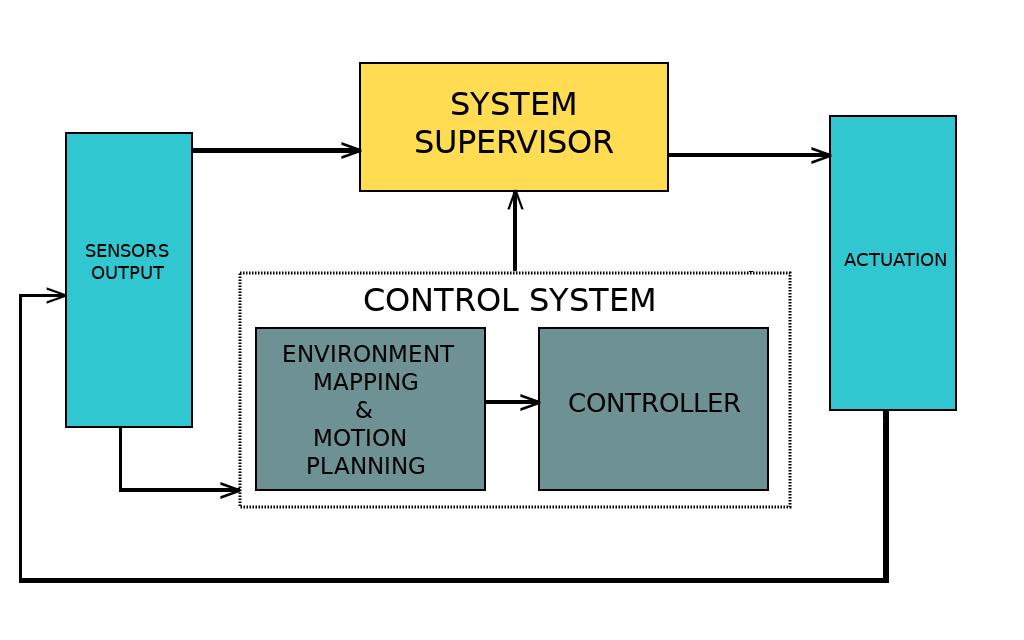
\includegraphics[width=\textwidth]{img/av-architecture.png}
	\caption{High-level abstraction of the system's software architecture}
\end{figure}

Data from sensors are inputs of the control system, here simplified as compose by two constituent systems: one in charge of collecting data directly from the sensors, process them in order to build an \textsl{occupancy grid}\footnote{A matrix mapping the environment, the cells $a_{i,j}$ are flagged with 0 if there's no object at coordinates $i,j$, 1 if occupied.} to map the surrounding area and to create a physical model of the environment in order to follow the correct route to the destination without crashing. The Controller (usually composed of a Velocity Controller\footnote{Controller in charge of adjusting the vehicle's speed} and a Steering Controller\footnote{Controller that determines the steering angle} uses these data to adjust the values on the actuator controlling the movements of the car: throttle, brake and steer.\newline
Due to the criticity of their task, it's mandatory to have a System Supervisor, a System in charge of detecting possible hardware failures or wrong outputs\footnote{With \textsl{"wrong"} is intended not only outputs out of the domain space but also outputs that would cause the system to fail (e.g. causing a crash)} from the Control System and, if needed, activate a corrective routine.

The System Supervisor is the main failure avoidance component of such systems. Of course there may be specific checks when data are processed, but the last decision is up to this system's monitor and the underestimation of its importance can lead to dramatic consequences, such as the 2018 accident in Arizona, where a woman was killed by a self-driving car.\cite{arizuber} Further inspections showed that the car's radar and lidar data detected the victim almost 6 seconds before the impact and it took 4 seconds circa to infer that there was an obstacle on the road and that an emergency brake was needed. However, this safety-checker was disabled during tests for "smoother rides", causing the accident.\cite{govarizuber}\newline\newline
The extreme complexity of these systems raise concerns among the experts: the way te system's safety is studied and tested must be looked from a new point of view and to sensitise about safety culture.\cite{koopman}


\section{Safety And Autonomous Vehicles}

According to a SAE International tentative to classify self-driving cars' autonomy, the level of automation can be divided in 6 tiers, ranging form 0 to 5. Level 0 means no autonomy: a human driver just drives the car, level 5 means that there's no need of human intervention at all and the car is not only capable of driving safely on the road, but it must be able to avoid catastrophic failures that may seriously harm (or kill) people.
The more autonomous the car is, the higher the dependability requirements are for it to be put on public roads.
It is well known that demonstrating a system's dependability is not an easy task for itself, it gets even harder with ultra-high dependability systems such as these are. In adition to the problem itself, demonstrating autonomous cars' dependability has two more problems to deal with: how to safely and effectively test the system and the need for neural networks to achieve the task.

Lots of studies demonstrated that it's unthinkable to just test cars on the roads. One of these, that we will refer to as the RAND Study, answers the question of how many mils of driving would it take to demonstrate autonomous vehicles' reliability using classical statistical inference, saying that if autonomous cars fatality rate was 20\% lower than humans', it would take more than 500 years with \textsl{"a fleet of 100 autonomous vehicles being test-driven 24 hours a day, 365 days a year at an average speed of 25 miles per hour"}.\cite{randstudy}\newline

The validation of ultra-high dependability requirements for safety-critical systems is a well known problem in safety literature and has not been introduced by the advent of autonomous cars. In fact, the RAND study is nothing but a specific case of the problem considered in a work published in 1993 by Littlewood \& Strigini, in which the same concepts (with a deeper level of detail) are discussed.\cite{littlewoodStrigini}\newline

The main problem with the RAND study approach is that future failures frequency can not be predicted just using the observed one. Not just for the quantitative results of the impossibility of it, but also because of this approach can not work: an observed frequency failure of 0 would lead to optimistic (and possibly harmful) predictions. Luckily, this problem is surmountable, as shown in \textsl{this}\cite{zhaoStrigini} work by Zhao et al.\newline\newline

Validating the dependability requirements of an autonomous car seems a hard task already. Things are made even harder by the fact that these cars are driven by neural networks.\newline
In these years there is a huge interest in the \textsl{machine learning} sector, and this has made that a lot of progress was done in the research. It's also thanks to these progresses that autonomous cars now seem like something we can achieve, since these AIs gave surprising results with their skills and big names such as \textsl{Uber} and \textsl{Tesla} are putting more and more efforts in AI research.

This new wave of AI research is deeply changing the way we interact with computer systems, and surprising results were achieved with neural networks.\newline
These tools have proven to outclass \textsl{"classic"} software solutions (intended as non-neural network) in a lot of tasks, ranging from \textsl{Object Detection}\cite{retinaNet} to \textsl{Gaming}\cite{alphaGo} problems, performing even better than humans.\cite{alphaGoBeatsMan}\newline

The complexity of the environment in which the system performs and the need of quick decision-making procedures and fast responses to events that \textsl{cannot} be planned with \textsl{"classic"} software, make neural networks the perfect tool to achieve the task of a car being able to drive by itself, thanks to their ability to handle multiple situations that were not explicitly written in the software. However, this raises serious issues about the safety of the whole system for many reasons.\newline

If neural networks gave promising results on one hand, and they seem the only way to achieve goals such as autonomous cars, on the other hand it has been shown many times how weird a network's prediction can get when \textsl{minimally} perturbating the inputs\cite{stupidnn} and how high the confidence interval can be.\cite{foolnn} The lack of official regulations and certifications of these kinds of software, as well as the need to truly understand neural networks, is raising concerns on how dependable these systems can be and consciousness is now growing on the topic, asking for more regulations on companies developing advanced AIs.\cite{elonmusk}\newline

\section{Controller - Checker Problem}

==============================================================================================

Qui descriverei il nostro problema. Per adesso ho solo copincollato quello che avevo scritto in precedenza, userei questa sezione per giustificare cosa facciamo

=================================================================================================


As the network learns, we expect the area covered by the Primary to grow. With a relatively simple Monitor, in relatively simple scenarios, there will potentially be no overlapping between the hazard areas covered by the two. In this phase, the safety gain provided by the use of a (correctly implemented) safety checker will be remarkable, since the Primary is still learning to handle "easy" demands. As pointed in the previous sections, our main goal is to observe and study the variation of the dependability provided by the monitor when the network is trained to handle "hard" demands, since there are no guarantees on the Monitor's performance in the long period.\newline
As noted in \cite{striginiPopov} the probability of a failure for a \textsl{system} composed by a \textsl{Primary Component} and a \textsl{Safety-Monitor} on a random demand X is:

\begin{equation}
P_{fp} (1 - Coverage_{\sigma}) - covariance_{Q} (\theta (X), C_{\sigma} (\sigma , X))
\end{equation}

where:

\begin{itemize}
	\item $P_{fp} (1 - Coverage_{\sigma})$ is the probability of a failure in the Primary Component ($P_{fp}$) that is \textbf{not detected} by the Safety Monitor (the term $1 - Coverage_{\sigma}$ is exactly the probability of having a false negative/positive)
	\item $covariance_{Q} (\theta (X), C_{\sigma}, X)$ given a demand profile $Q = <x, y>$ (i.e. the pair <demand, output), measures the correlation between:
	\begin{itemize}
		\item[$\theta (X)$ -] The expected probability that the Primary will fail when processing demand $X$
		\item[$C_{\sigma} (\sigma, X)$ -] the term identifying the \textsl{Coverage Factor} of the \textbf{Monitor}, on the specific demand $X$
	\end{itemize}
\end{itemize}

This formula highlights the deep connection between the safety levels of the Controller and the Monitor, when it comes to the global safety of the system. It is clear from the equation that the probability of observing a failure in the system is also depending on the specific demand $X$, that's 
.\newline

***************\newline

TO REVIEW:\newline

***************\newline

The formula points the fact that to have the probability of observing a failure in the system depends not only on \textsl{all the possible demands} in the \textsl{demand space} but also on how the controller and the monitor react to them.\newline


